\documentclass[conference]{IEEEtran}

\usepackage[utf8]{inputenc}
\usepackage[T1]{fontenc}
\usepackage{silence}\WarningsOff[latexfont]

\usepackage{amsmath}

\RequirePackage{tikz}[2010/10/13]
\usetikzlibrary{arrows,automata,calc,intersections,patterns,decorations.pathmorphing,decorations.pathreplacing}

\usepackage{graphicx}
\usepackage{cite}
\usepackage{url}
\usepackage[caption=false,font=footnotesize]{subfig}
\usepackage[binary-units,per-mode=symbol]{siunitx}
\sisetup{list-final-separator = {, and }}
\usepackage{booktabs}
\usepackage{pifont}
\usepackage{microtype}
\usepackage{textcomp}
\usepackage[american]{babel}
\usepackage[noabbrev,capitalise]{cleveref}
\usepackage{xspace}
\usepackage{hyphenat}
\usepackage[draft,inline,nomargin,index]{fixme}
\fxsetup{theme=color}
\usepackage{grffile}
\usepackage{xfrac}
\usepackage{multirow}
\RequirePackage{xstring}
\RequirePackage{xparse}
\usepackage{float}
\usepackage{blkarray}
\usepackage{amsmath}

\RequirePackage[index=true]{acro}
\NewDocumentCommand\acrodef{mO{#1}mG{}}{\DeclareAcronym{#1}{short={#2}, long={#3}, #4}}
\NewDocumentCommand\acused{m}{\acuse{#1}}
\usepackage{upquote}

\acrodef{WSN}{Wireless Sensor Network}
\acrodef{MANET}{Mobile Ad Hoc Network}
\acrodef{ROI}{Region of Interest}{short-indefinite={an}, long-plural-form={Regions of Interest}}

\begin{document}

\title{Devising a Model}

\author{
	\IEEEauthorblockN{Rodrigo Joni Sestari, Mat. number 179020}
	\texttt{rodrigo.sestari@studenti.unitn.it}
}

\maketitle

\begin{abstract}
This report describes a simply model that represents the Python Simulator Extension described in the previous report.

\end{abstract}

\acresetall

\section{Introduction}
\label{sec:introduction}

\begin{itemize}
\item general motivation is create a model that represents the simulator.
\item problem: is modelling a trivial a carrier sensing in the network.
\item strategy: use a continuous time Markov chain CTMC to modelling it.
\end{itemize}



\section{Basic Information}

The first propose a very simple model the result will compared with the simulator extension, the second step will improve it to be a bit more realistic.
 
 

\section{The System Model}

\subsection{assumptions}
\begin{itemize}
\item The network is composed by 10 nodes where all node are visible by all.
\item The distance between the nodes not affects the transmission.
\item Transmission speed is constant.
\item One channel of communication.
\end{itemize}



\subsection{modeling}


Considering all possible events that may occur in a network, CTMC was chosen to modelling it. Was identified the set of variables that represent the state of the system, in this case the states are the transmission nodes, it was enumerates from 1 to 10, when happens a collision, the packets are lost, its no longer part of the throughput, then was created a new state called \textit{1 collision}.

\\The parameters \( \lambda \)  indicates the arrival rates for packets  in seconds, it is exponentially distributed inter-arrival times with  \( \lambda \) from 10 to 1510 arrivals/s. The service rate is constant in packets/s, indicate by  \( \mu \), It is the average of served packets, that is, the transmission speed divided by the average size of a packet: \( (8 *1024^2) / ((32+1460)*8/2) \).

\bigskip


\begin{figure}[H]
	\centering	 
	\subfloat{\label{fig:md1}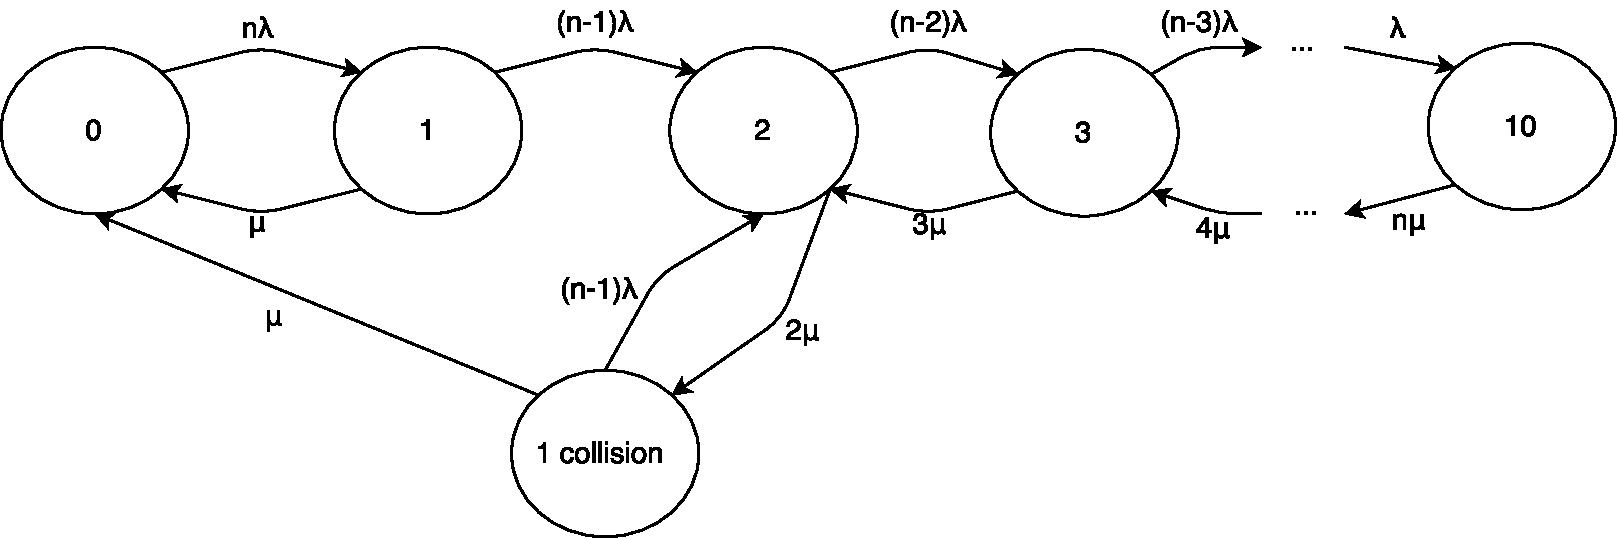
\includegraphics[width=\columnwidth]{figures/rede_1.pdf}}
	\caption{Shows a CTMC model representing the states of the system}%
\end{figure}

The states and parameters of the CTMC model are summarized here:

\begin{itemize}
\item 0: indicate the network in state Iddle.
\item 1..10: stations transmitting.
\item 1 collision: indicate the network collision.
\item \( \lambda \): arrival rate.
\item  \( \mu \): service rate.
\item n: total nodes.
\end{itemize}
 


\subsection{CTMC transition matrix}

A CTMC can simply be described by a transition matrix  \( P = P_{ij} \), describing how the chain changes state step-by-step at transition epochs.
\\

 \resizebox{0.9\linewidth}{!}{%
\begin{equation_1}
  \mathbf{Q}=
  \begin{blockarray}{*{7}{c} l}
    \begin{block}{*{7}{>{$\footnotesize}c<{$}} l}
      0 & 1 & 1c & 2 & 3 & ...  & 10   \\
    \end{block}
    \begin{block}{[*{7}{c}]>{$\footnotesize}l<{$}}
      0 & 10\lambda & 0 & 0 & 0 & ...  & 0 &   0 \\
      \mu & 0 & 9\lambda & 0& 0 & ...  & 0 &   1 \\
      \mu & 0 & 0 &9\lambda  & 0 & ...  & 0 &   1c \\
	  0 & 0 & 2\mu & 0 &8\lambda & ...  & 0 &   2 \\
	  0 & 0 & 0 & 3\mu & 0 & 7\lambda & 0 &  3 \\
	    ... & ... & ... & ...  & 4\mu & ... & \lambda & ...\\
	  0 & 0 & 0 & 0 & 0 & 10\mu & 0 &  10\\

    \end{block}
  \end{blockarray}
\end{equation_1}
}

\subsection{Infinitesimal generator matrix}
This matrix is called the infinitesimal generator of the Markov chain. Clearly, this matrix determines the transition probabilities of the Markov chain. This is defined by the following properties:
\bigskip
\begin{enumerate}
\item \( 0 \leq -q_{ii} < \infty  \)
\item \( 0 \leq q_{ij} :\) for all \( i \neq j  \)
\item \( \sum_j q_{ij} = 0 :\) for all \( i \)

\end{enumerate}


\bigskip

 \resizebox{0.95\linewidth}{!}{%
\begin{equation_2}
  \mathbf{Q}=
  \begin{blockarray}{*{7}{c} l}
    \begin{block}{*{7}{>{$\footnotesize}c<{$}} l}
      0 & 1 & 1c & 2 & 3 & ...  & 10   \\
    \end{block}
    \begin{block}{[*{7}{c}]>{$\footnotesize}l<{$}}
      -(10\lambda) & 10\lambda & 0 & 0 & 0 & ...  & 0 &   0 \\
      \mu & -(\mu + 9\lambda) & 9\lambda & 0& 0 & ...  & 0 &   1 \\
      \mu & 0 & -(\mu + 9\lambda) &9\lambda  & 0 & ...  & 0 &   1c \\
	  0 & 0 & 2\mu & -(2\mu + 8\lambda) &8\lambda & ...  & 0 &   2 \\
	  0 & 0 & 0 & 3\mu & -(3\mu + 7\lambda) & 7\lambda & 0 &  3 \\
	    ... & ... & ... & ...  & 4\mu & -(4\mu + \lambda) & \lambda & ...\\
	  0 & 0 & 0 & 0 & 0 & 10\mu & -(10\mu) &  10\\

    \end{block}
  \end{blockarray}
\end{equation_2}
}

\subsection{Steady-state Distribution}

The chain is irreducible and recurrent. To theoretically find the steady state distribution, we have to solve the balance equations: \( pQ=0  \) with the constraint  \(  \sum_{i} {p_^{i}}=1   \) There are \( dim(Q) - 1 \)  independent columns, so the latter constraint is equivalent to substitute any column by ones and match it to one at the other side of the equation. The solution  \( p \) represents the probability of being at each state in the long-term, that is:
 
 

\bigskip

 \resizebox{0.95\linewidth}{!}{%
\begin{equation_2}
  \mathbf{\( p. \)}
  \begin{blockarray}{*{7}{c} l}
    \begin{block}{*{7}{>{$\footnotesize}c<{$}} l}
      0 & 1 & 1c & 2 & 3 & ...  & 10   \\
    \end{block}
    \begin{block}{[*{7}{c}]>{$\footnotesize}l<{$}}
      1 & 10\lambda & 0 & 0 & 0 & ...  & 0 &   0 \\
      1 & -(\mu + 9\lambda) & 9\lambda & 0& 0 & ...  & 0 &   1 \\
      1 & 0 & -(\mu + 9\lambda) &9\lambda  & 0 & ...  & 0 &   1c \\
	  1 & 0 & 2\mu & -(2\mu + 8\lambda) &8\lambda & ...  & 0 &   2 \\
	  1 & 0 & 0 & 3\mu & -(3\mu + 7\lambda) & 7\lambda & 0 &  3 \\
	    1 & ... & ... & ...  & 4\mu & -(4\mu + \lambda) & \lambda & ...\\
	  1& 0 & 0 & 0 & 0 & 10\mu & -(10\mu) &  10\\

    \end{block}
  \end{blockarray} = (1,0,0,0,0,...,0)
\end{equation_2}
}

 
\bigskip 
The steady-state probabilities   \( \pi_{i} \)  may be interpreted as the proportion of time that the CTMC spends in state  \(i \), where  \(i \in \left\{  0, 1,1c, 2,3,4,5,6,7,8,9,10\right\}\).
The objective is know the  throughput, so we need discovery how long time the system stay in the state \( \pi_{ 1 } \). The arrivals in this case is given by \(\lambda*\) \(\pi_{ 1 }\).

\bigskip

\section{The model improvement}

In the \textit{Base model}, only the state 2 leads to the collision state \textit{1 collision}, we can have collisions also in the states 3..10, the improvement model consist, in to create collision states for the other nodes.

\begin{figure}[H]
	\centering	 
	\subfloat{\label{fig:md1}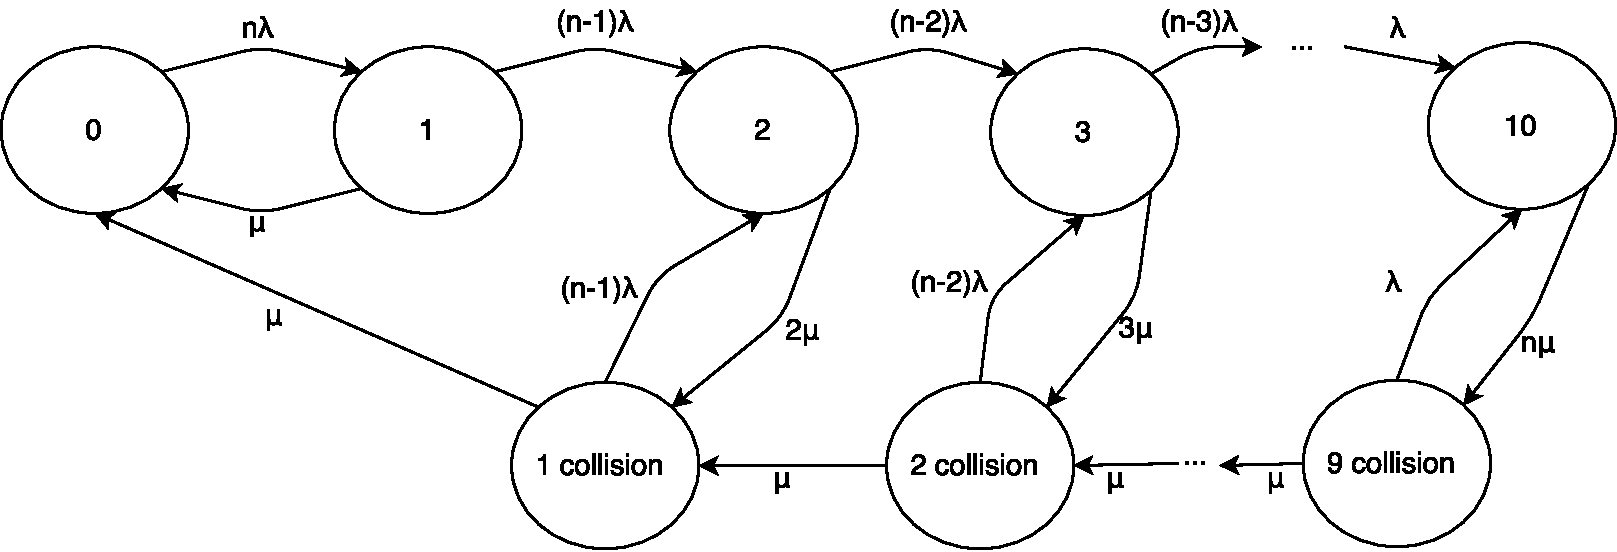
\includegraphics[width=\columnwidth]{figures/rede_2.pdf}}
	\caption{The model improvement}%
\end{figure}


\section{Considerations}

The Figure 3 shows the comparison between the two models developed in this document with the Simulator mean throughput using only one seed. The \textit{Base model} throughput is slightly higher than the \textit{Model improvement}, but the throughput drop after reaching the peak is highest in relation to the \textit{Model improvement}. This happens because in the \textit{Model improvement}, the system stays more time in the collision states \textit{1..9 collision}, making the \textit{Model improvement} more realistc than the \textit{Base model}. 
\bigskip

\begin{figure}[H]
	\centering	 
	\subfloat{\label{fig:md1}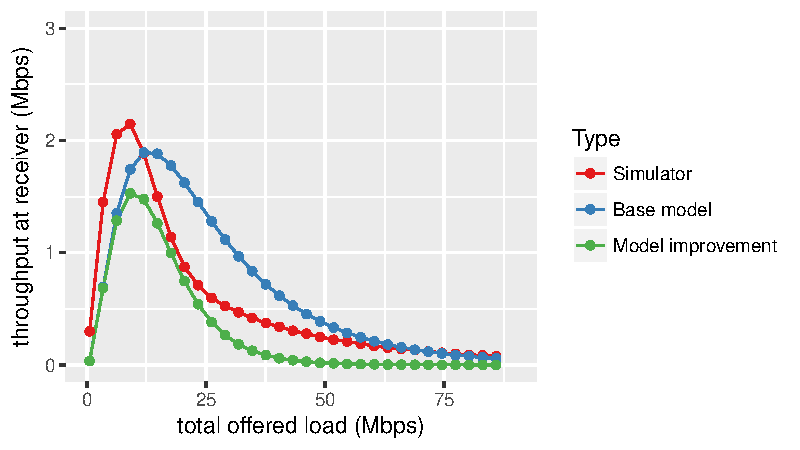
\includegraphics[width=\columnwidth]{figures/modelMEANthr.pdf}}
	\caption{comparison between simulation and models}%
\end{figure}



\end{document}
